%%
%% This is file `sample-sigconf.tex',
%% generated with the docstrip utility.
%%
%% The original source files were:
%%
%% samples.dtx  (with options: `all,proceedings,bibtex,sigconf')
%% 
%% IMPORTANT NOTICE:
%% 
%% For the copyright see the source file.
%% 
%% Any modified versions of this file must be renamed
%% with new filenames distinct from sample-sigconf.tex.
%% 
%% For distribution of the original source see the terms
%% for copying and modification in the file samples.dtx.
%% 
%% This generated file may be distributed as long as the
%% original source files, as listed above, are part of the
%% same distribution. (The sources need not necessarily be
%% in the same archive or directory.)
%%
%%
%% Commands for TeXCount
%TC:macro \cite [option:text,text]
%TC:macro \citep [option:text,text]
%TC:macro \citet [option:text,text]
%TC:envir table 0 1
%TC:envir table* 0 1
%TC:envir tabular [ignore] word
%TC:envir displaymath 0 word
%TC:envir math 0 word
%TC:envir comment 0 0
%%
%%
%% The first command in your LaTeX source must be the \documentclass
%% command.
%%
%% For submission and review of your manuscript please change the
%% command to \documentclass[manuscript, screen, review]{acmart}.
%%
%% When submitting camera ready or to TAPS, please change the command
%% to \documentclass[sigconf]{acmart} or whichever template is required
%% for your publication.
%%
%%
% \documentclass[sigconf, screen, review]{acmart}
% \documentclass[sigconf]{acmart
% \documentclass[sigconf, 9pt]{acmart}
% Updated to what the Conf wanted
\documentclass[manuscript, review=true, screen=true, sigconf,natbib=true, anonymous]{acmart}
\settopmatter{printacmref=false} % Removes citation information below abstract
\setcopyright{none}              % Removes copyright box
\renewcommand\footnotetextcopyrightpermission[1]{} % Removes footnote with conference information in first column
\pagestyle{plain}                % Removes running headers on subsequent pages

%%
%% \BibTeX command to typeset BibTeX logo in the docs
\AtBeginDocument{%
  \providecommand\BibTeX{{%
    Bib\TeX}}}

\usepackage{url}
\usepackage{graphicx}
\usepackage{subcaption}
\usepackage{array}
\usepackage{booktabs}
\usepackage{multirow}
\usepackage{caption}
\usepackage{makecell}
\usepackage{geometry}
\usepackage{svg}
\usepackage{float}
\usepackage{enumitem}
\usepackage{algorithm}
\usepackage{stfloats}
\usepackage[noend]{algpseudocode}
\usepackage[htt]{hyphenat}


%% Rights management information.  This information is sent to you
%% when you complete the rights form.  These commands have SAMPLE
%% values in them; it is your responsibility as an author to replace
%% the commands and values with those provided to you when you
%% complete the rights form.
\setcopyright{none} 
%\setcopyright{acmlicensed}
% \copyrightyear{2026}
% \acmYear{2026}
% \acmDOI{XXXXXXX.XXXXXXX}

%% These commands are for a PROCEEDINGS abstract or paper.
% \acmConference[MICRO 2026]{The 58th IEEE/ACM International Symposium on Microarchitecture}{October 31--November 04, 2026}{Athens, Greece}
%%
%%  Uncomment \acmBooktitle if the title of the proceedings is different
%%  from ``Proceedings of ...''!
%%
%%\acmBooktitle{Woodstock '18: ACM Symposium on Neural Gaze Detection,
%%  June 03--05, 2018, Woodstock, NY}

% \acmISBN{978-X-XXXX-XXXX-X/XX/XX}


%%
%% Submission ID.
%% Use this when submitting an article to a sponsored event. You'll
%% receive a unique submission ID from the organizers
%% of the event, and this ID should be used as the parameter to this command.
%%\acmSubmissionID{123-A56-BU3}

%%
%% For managing citations, it is recommended to use bibliography
%% files in BibTeX format.
%%
%% You can then either use BibTeX with the ACM-Reference-Format style,
%% or BibLaTeX with the acmnumeric or acmauthoryear sytles, that include
%% support for advanced citation of software artefact from the
%% biblatex-software package, also separately available on CTAN.
%%
%% Look at the sample-*-biblatex.tex files for templates showcasing
%% the biblatex styles.
%%

%%
%% The majority of ACM publications use numbered citations and
%% references.  The command \citestyle{authoryear} switches to the
%% "author year" style.
%%
%% If you are preparing content for an event
%% sponsored by ACM SIGGRAPH, you must use the "author year" style of
%% citations and references.
%% Uncommenting
%% the next command will enable that style.
%%\citestyle{acmauthoryear}
\settopmatter{printfolios=true}
\settopmatter{printacmref=false}
%\pagestyle{plain}

% \newcommand{\Ryzen}{AMD Ryzen\textsuperscript{\texttrademark}~}
% \newcommand{\Ryzen}{AMD Ryzen}

%%
%% end of the preamble, start of the body of the document source.
\begin{document}

\setlist[itemize]{noitemsep, topsep=12pt}

% \newcommand{\eddie}[1]{\textcolor{orange}{[EDDIE: #1]}}

% setthis to remove comments
% \renewcommand{\eddie}[1]{}

%%
%% The "title" command has an optional parameter,
%% allowing the author to define a "short title" to be used in page headers.
\title{ExpertAhead: Latency-Hiding Expert Prediction for SSD-Backed MoE Inference on Unified-Memory Edge Devices}
% \subtitle{\normalsize{ASP\_DAC 2026 Submission
%     -- Confidential Draft -- Do NOT Distribute!!}}
%%
%% The "author" command and its associated commands are used to define
%% the authors and their affiliations.
%% Of note is the shared affiliation of the first two authors, and the
%% "authornote" and "authornotemark" commands
%% used to denote shared contribution to the research.
% Commented due to double blind: Placeholder
% \author{\normalsize{Michael Gamota} \, \, \, \, \normalsize{Gregory Jun} \, \, \, \, \normalsize{Deming Chen}}

%%
%% By default, the full list of authors will be used in the page
%% headers. Often, this list is too long, and will overlap
%% other information printed in the page headers. This command allows
%% the author to define a more concise list
%% of authors' names for this purpose.

%%
%% The abstract is a short summary of the work to be presented in the
%% article.

%%%%%% -- PAPER CONTENT STARTS-- %%%%%%%%

\begin{abstract}
Mixture-of-Experts (MoE) LLM architectures enable large-scale models with sparse per-token computation, making them attractive for SSD-backed inference on memory-constrained unified-memory edge systems, where inactive experts can be offloaded to the SSD. However, SSD access latency is typically at least an order of magnitude higher than memory latency, causing decode throughput to become dominated by expert loading. Existing MoE acceleration techniques typically rely on predictive prefetching, cache-aware routing, or optimized cache management, but the interaction between these techniques on SSD-backed unified-memory edge platforms remains underexplored. Furthermore, expert prediction methods face a tradeoff between prediction horizon and resource overhead: lightweight short-horizon predictors provide limited opportunities to hide SSD latency, while long-horizon approaches, often relying on speculative decoding with draft models, introduce substantial memory overhead.

We propose \textbf{ExpertAhead}, a lightweight transformer-based expert predictor that forecasts expert activations across multiple future decoding steps, enabling proactive SSD prefetching with minimal memory overhead. We evaluate our runtime on an AMD Ryzen AI 9 HX 370 (Strix Point) SoC, where model inference executes on the integrated GPU while expert prediction and SSD scheduling execute concurrently on the CPU, leveraging the platform's unified-memory architecture to overlap computation and storage transfers. An oracle predictor integrated into the same runtime as ExpertAhead, with perfect precision and recall, achieves up to 3.11$\times$ speedup over an equal-memory baseline that uses no predictive prefetching and a random eviction policy. \textbf{ExpertAhead} achieves 1.65$\times$ speedup over this baseline with lossless inference. \textbf{ExpertAhead-CC}, which integrates prediction with cache-conditional routing, further improves throughput, achieving 2.05$\times$ speedup with a small increase in perplexity.
\end{abstract}
%%
%% The code below is generated by the tool at http://dl.acm.org/ccs.cfm.
%% Please copy and paste the code instead of the example below.
%%
%\begin{CCSXML}
%<ccs2012>
% <concept>
%  <concept_id>00000000.0000000.0000000</concept_id>
%  <concept_desc>Do Not Use This Code, Generate the Correct Terms for Your Paper</concept_desc>
%  <concept_significance>500</concept_significance>
% </concept>
% <concept>
%  %<concept_id>00000000.00000000.00000000</concept_id>
%  <concept_desc>Do Not Use This Code, Generate the Correct Terms for Your Paper</concept_desc>
%  <concept_significance>300</concept_significance>
% </concept>
% <concept>
%  %<concept_id>00000000.00000000.00000000</concept_id>
%  <concept_desc>Do Not Use This Code, Generate the Correct Terms for Your Paper</concept_desc>
%  <concept_significance>100</concept_significance>
% </concept>
% <concept>
 % <concept_id>00000000.00000000.00000000</concept_id>
%  <concept_desc>Do Not Use This Code, Generate the Correct Terms for Your Paper</concept_desc>
%  <concept_significance>100</concept_significance>
% </concept>
%</ccs2012>
%\end{CCSXML}

%\ccsdesc[500]{Do Not Use This Code~Generate the Correct Terms for Your Paper}
%\ccsdesc[300]{Do Not Use This Code~Generate the Correct Terms for Your Paper}
%\ccsdesc{Do Not Use This Code~Generate the Correct Terms for Your Paper}
%\ccsdesc[100]{Do Not Use This Code~Generate the Correct Terms for Your Paper}

%%
%% Keywords. The author(s) should pick words that accurately describe
%% the work being presented. Separate the keywords with commas.



% \keywords{large language models, mixture of experts, edge AI, prediction}

\maketitle
\pagestyle{plain} % MUST come exactly after \maketitle
% \newpage
\section{Introduction}

Mixture-of-Experts (MoE) large language model (LLM) architectures enable large parameter counts while activating only a subset of those parameters during each decode step. This creates opportunities for the deployment of MoE models on memory-constrained platforms by offloading some or all of the inactive experts to SSD. However, SSD access latency is typically at least an order of magnitude higher than memory access latency, causing decode throughput in SSD-backed MoE inference to become heavily dominated by expert loading latency.

Existing MoE inference acceleration techniques primarily address this bottleneck by overlapping computation with predictive prefetching, reducing overall SSD traffic by modifying expert selection decisions, or optimizing expert cache management. However, most expert prefetching approaches target conventional accelerator memory hierarchies, such as transferring experts between host memory and discrete GPU memory \cite{xue2025moeinfinityefficientmoeinference,gavhane2025moebeyondlearningbasedexpertactivation,song2025promoefastmoebasedllm}, rather than SSD-backed unified-memory (UMA) edge systems where expert loading involves substantially higher latency and limited memory capacity. Cache-conditional routing \cite{skliar2025mixturecacheconditionalexpertsefficient, zhu2026smoealgorithmsystemcodesignpushing} reduces total expert loads by modifying expert selection decisions, but introduces a tradeoff with model output quality. Furthermore, the interaction between predictive prefetching, cache-aware routing, and cache management policies remains underexplored for UMA edge platforms.

Additionally, existing predictive prefetching methods generally fall into two categories: lightweight short-horizon predictors \cite{zhu2025preattentionexpertpredictionprefetching, eliseev2023fastinferencemixtureofexpertslanguage, zhu2026daliworkloadawareoffloadingframework, fang2025fatefastedgeinference, yao2024exploitinginterlayerexpertaffinity, song2025promoefastmoebasedllm, zhang2026duoservemoedualphaseexpertprefetch, yi2025edgemoeempoweringsparselarge, gavhane2025moebeyondlearningbasedexpertactivation,xue2025moeinfinityefficientmoeinference}, which provide a limited hiding window for prefetches, and long-horizon approaches \cite{wang2025moespeqspeculativequantizeddecoding, chen2025spmoespeculativedecodingprefetching}, often enabled through draft models within speculative decoding frameworks, which require substantial memory overhead. This work explores the middle ground between these approaches with ExpertAhead, a transformer-based expert predictor that uses token embeddings, prior expert-usage statistics, and prefill expert activations to predict future expert activations across multiple decoding steps. We first characterize the theoretical performance of expert prediction with an oracle and then design a practical predictor optimized for SSD-backed MoE inference. We further integrate ExpertAhead with cache-conditional routing to develop ExpertAhead-CC, which jointly exploits prediction and adaptive expert selection.

We evaluate our system on an AMD Ryzen AI 9 HX 370, a UMA SoC, where model inference executes on the integrated GPU while expert prediction and SSD scheduling execute concurrently on the CPU. An oracle predictor using identical scheduling to ExpertAhead achieves up to 3.11$\times$ decode speedup over a random-eviction equal-memory baseline. ExpertAhead achieves 1.65$\times$ speedup over that same baseline, and ExpertAhead-CC achieves 2.05$\times$ speedup with a small increase in perplexity.  Our contributions include:
\begin{itemize}[leftmargin=1.5em] 
    \item \textbf{Lightweight expert predictor:} We train and evaluate a predictor that leverages contextual information to predict future expert usage, targeting SSD-backed UMA MoE inference. We report  3.11$\times$ speedup over an equal-memory baseline with an oracle predictor to motivate this prediction paradigm.
    
    \item \textbf{End-to-end SSD-backed MoE inference framework:} We integrate predictive prefetching, cache-conditional routing, and an expert cache management policy into a complete inference system and evaluate their combined impact through ExpertAhead-CC, achieving 2.05$\times$ speedup over an equal-memory baseline. 
    
    \item \textbf{Modeling SSD-backed decode:} We develop analytical models describing the relationship between storage and compute latency, prediction stride, cache size, prefetch budget, and per-token latency for SSD-backed decode. 
\end{itemize}
 
% \newpage
\section{Background and Related Work}

\begin{figure}[t]
    \vspace{-5pt}
    \centering
    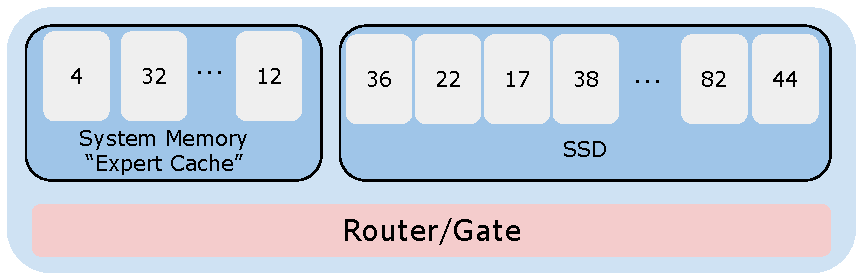
\includegraphics[width=\columnwidth]{figures/expert_storage_cropped.pdf}
    \vspace{-10pt}
    \caption{Selected experts may reside in memory or SSD}
    \label{fig:transformer_vs_moe}
    \vspace{-5pt}
\end{figure}

\subsection{Hardware Architecture and Constraints}
Modern edge AI platforms, \cite{amd-2025-ryzen-ai-9-hx-370,feng2025profilingapplesiliconperformance,snapdragonX,LunarLake}, employ a Unified Memory Architecture (UMA) in which the CPU, integrated GPU (iGPU), and other compute units share a common physical memory pool. Unlike discrete GPU systems, where host-to-device transfers often dominate MoE inference latency \cite{xue2025moeinfinityefficientmoeinference,gavhane2025moebeyondlearningbasedexpertactivation,song2025promoefastmoebasedllm}, UMA eliminates explicit host-to-device transfers in most cases through shared memory. However, when MoE models exceed available memory capacity and inactive experts are offloaded to an SSD, decode throughput becomes bottlenecked by expert loading latency from SSD  \cite{kim2026flashmoereducingssdio}.

\subsection{SSD-Backed MoE Inference}
MoE architectures \cite{shazeer2017outrageouslylargeneuralnetworks,zhang2022moeficationtransformerfeedforwardlayers,fedus2022switchtransformersscalingtrillion} trade the single dense feed-forward network (FFN) found in classical transformer models \cite{vaswani2017attention} for many router-selected, smaller FFNs (experts). Although sparse activation primarily reduces per-token computation, it also allows inactive experts to be offloaded to secondary storage, making deployment of large MoE models feasible on memory-constrained systems. Recent work has studied SSD-backed inference to explore this opportunity. For example, FlashMoE \cite{kim2026flashmoereducingssdio} directly addresses the SSD I/O bottleneck by employing ML-based cache replacement policies to keep the most relevant experts resident in memory. While somewhat effective, this is a reactive cache policy optimization; in contrast, ExpertAhead performs proactive, asynchronous SSD prefetches, allowing the system to actively hide load latency on top of implementing an expert cache management policy.

\subsection{Expert Prediction and Prefetching}
Expert prefetching is a widely studied technique for accelerating MoE inference, most commonly deployed to move experts from host CPU memory into discrete GPU memory \cite{xue2025moeinfinityefficientmoeinference,gavhane2025moebeyondlearningbasedexpertactivation,song2025promoefastmoebasedllm,zhu2025preattentionexpertpredictionprefetching, zhang2025daopdataawareoffloadingpredictive}. 

Existing prefetching approaches can be classified by their prediction horizon. \textbf{Short-horizon methods} operate intralayer: predicting expert usage within the same layer for the current token \cite{zhu2025preattentionexpertpredictionprefetching}, or interlayer: predicting activations in future layers. Interlayer prediction has been studied by applying a future layer's gating function directly to current hidden states \cite{eliseev2023fastinferencemixtureofexpertslanguage, zhu2026daliworkloadawareoffloadingframework, fang2025fatefastedgeinference, yao2024exploitinginterlayerexpertaffinity}, utilizing offline-trained predictors \cite{song2025promoefastmoebasedllm, zhang2026duoservemoedualphaseexpertprefetch, yi2025edgemoeempoweringsparselarge, gavhane2025moebeyondlearningbasedexpertactivation}, or leveraging an Expert Activation Matrix (EAM) \cite{xue2025moeinfinityefficientmoeinference}. Conversely, \textbf{long-horizon methods} extend the prediction window across multiple future tokens, typically by leveraging speculative decoding \cite{wang2025moespeqspeculativequantizeddecoding, chen2025spmoespeculativedecodingprefetching} to predict tokens and expert activations. However, the memory overhead required to maintain a secondary draft model makes this approach poorly suited for memory-constrained edge deployments. Allocating memory for this draft model reduces memory available for caching experts, which increases SSD accesses, the fundamental bottleneck, potentially offsetting the latency benefits of speculative decoding.

% For example, storing a draft model of the same relative size as used in \cite{chen2025spmoespeculativedecodingprefetching} would yield a 41\% decode slowdown compared to an equal-memory expansion of the expert cache in our system.

ExpertAhead occupies a practical middle ground: we utilize a lightweight predictor model to forecast expert usage for the next $S$ tokens. This multi-token horizon provides significantly more time to hide SSD loading latency than short-horizon methods, while avoiding the memory overhead of speculative draft models.

\subsection{Modified Expert Activation}
Beyond prefetching, reducing the volume of required expert loads is critical. Current approaches achieve this by pruning or dropping unimportant experts \cite{chen2022taskspecificexpertpruningsparse, qiu2025demonsdetailimplementingload} or by dynamically substituting router-selected SSD-resident experts to avoid disk reads \cite{skliar2025mixturecacheconditionalexpertsefficient, zhu2026smoealgorithmsystemcodesignpushing}. However, relying solely on cache-aware routing inherently limits model quality by not using all of the router-selected experts. Inspired by the evaluation framework in SpecMD \cite{hoang2026specmdcomprehensivestudyspeculative}, which assesses the combination of predictive and reactive techniques, ExpertAhead-CC implements predictive prefetching with cache-conditional routing. This ensures the system only substitutes an expert when it is not predicted or prefetched in time, thereby maximizing throughput while minimizing perplexity degradation.
% \newpage
\section{System Modeling and Design}

\subsection{Modeling Steady-State Decode}
\label{sec:modeling_decode}

We present a latency model for LLM decode under three expert management strategies: naive caching, predictive prefetching, and cache-conditional routing.  

We define the following quantities. Qwen3-30B-A3B \cite{yang2025qwen3technicalreport} has $L = 48$ MoE layers, each activating $K = 8$ of 128 experts per layer per token, giving $E = K \cdot L = 384$ expert invocations per token. Each expert is the same size, which for the quantized version, Qwen3-30B-A3B-AWQ~\cite{QuixiAIQwen3AWQ}, is $\sim$2.5 MB. We denote by $T_{ceil}$ the per-token latency when all experts are resident in unified system memory, including both the time spent loading weights from unified memory to the iGPU and compute time. Each expert that must be loaded from SSD incurs a cost $T_{SSD, n}$ , where $n$ is the number of concurrent expert loads. The analytical models in this section assume that background SSD transfers do not interfere with inference compute. 

\subsubsection{Baseline SSD-Backed Decode Model}
\label{sec:baseline_model}

We first model a baseline decode implementation in which expert loads are fully synchronous. For each expert invocation, the expert request either hits in the unified memory expert cache or misses and stalls the decode thread until the expert is fetched from SSD. Let $h \in [0,1]$ be the cache hit rate, so that the number of blocking misses per token is $E_{miss} = E \cdot (1 - h)$. The per-token latency is

\begin{equation}
    T_{0} = T_{ceil} +  E_{miss} \cdot T_{SSD,n}.
    \label{eq:lru}
\end{equation}

This model assumes that each blocking expert load contributes independently to decode latency and that SSD transfers cannot overlap with computation and always block the decode path. Figure~\ref{fig:timeline_blocking} illustrates this process with a toy 2-layer MoE LLM.

\begin{figure}[h]
    \centering
    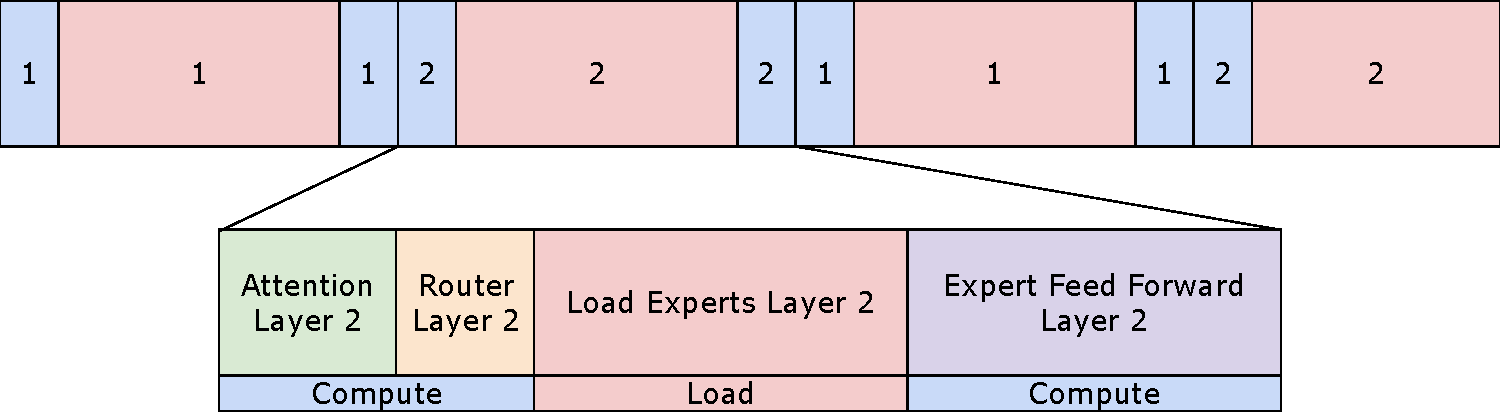
\includegraphics[width=\columnwidth]{figures/timeline_LRU_cropped.pdf}
    \vspace{-10pt}
    \caption{Timeline of decode with blocking expert loads. No predictive prefetch leads to reactive SSD loads on misses}
    \label{fig:timeline_blocking}
\end{figure}


\subsubsection{Predictive Prefetching} 
\label{sec:prefetch}

Predictive prefetching aims to reduce blocking loads by loading predicted experts into a per-layer expert cache of size $C$ proactively: the predictor has a stride, $S$, such that it fires once every $S$ tokens, and issues asynchronous SSD loads for experts likely to be used to generate the next $S$ tokens. If the loads finish before those experts are needed, they are already resident in the cache and no blocking stalls occur, as illustrated in Figure~\ref{fig:timeline_prefetch}. 

On each predictor invocation, up to $B$ prefetch loads (prefetch budget) are issued per layer, for a total issue budget of $M_{issue} = L \cdot B$ loads every $S$ tokens. Not all issued loads are useful: let $\pi \in [0,1]$ be the \emph{precision}, the fraction of prefetched experts that actually get requested by the router. Conversely, let $\rho \in [0,1]$ be the \emph{recall}, the fraction of experts that will be requested by the router on subsequent decode steps that the predictor correctly identified. Low precision wastes SSD bandwidth on unneeded loads; low recall increases cache misses, causing blocking loads from SSD. 

After the predictor runs, the ideal theoretical window to hide asynchronous SSD loads is  $S \cdot T_{ceil}$ ms, the compute time of the next $S$ tokens. This assumes an ideal predictive prefetching schedule where the earliest activated experts are loaded first. It should be noted that if all layers are issuing loads, we will saturate SSD bandwidth and cannot use the entire $S \cdot T_{ceil}$ ms window. We assume no bandwidth contention and that each expert takes $T_{SSD,n}$ ms to load, giving a maximum load hiding capacity:

\begin{equation}
    M_{cap} = \frac{S \cdot T_{ceil} }{T_{SSD, n}}.
    \label{eq:mcap}
\end{equation}

Let $U(S)$ be the number of expert misses that will occur over the next $S$ tokens. There are four constraining dimensions which limit how many experts can be successfully prefetched (hidden and correct) during the decode process of the next $S$ tokens:
\begin{enumerate}
\label{list:constraints}
    \item $\rho \cdot U(S) $: Number of future router requests that are predicted, not including those already in the cache
    \item $\pi \, L B $: Number of useful predictions that are issued, not including predicted experts already in the cache 
    \item $M_{cap}$: The number of prefetches that can complete within the available overlap window
    \item $C$: Number of experts that can be stored in the unified memory expert cache
\end{enumerate}

% This allows us to construct 

% \begin{equation}
%     M_{prefetch} = \min\!\left(\rho \, U(S) \cdot (1-h),\; \pi \, L B \cdot (1-h),\; M_{cap}, \, C\right).
%     \label{eq:mprefetch}
% \end{equation}


\begin{figure}[h]
    \centering
    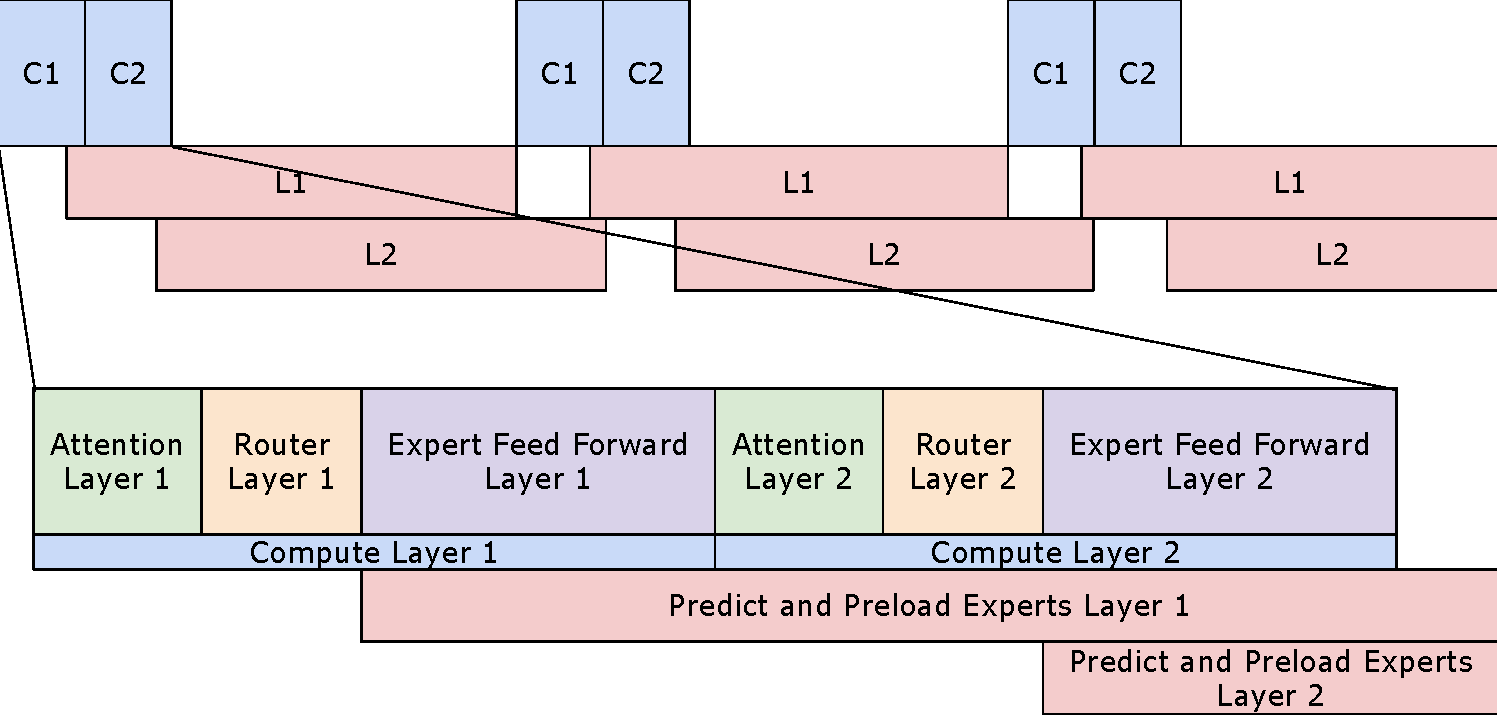
\includegraphics[width=\columnwidth]{figures/timeline_prefetch_cropped.pdf}
    \vspace{-10pt}
    \caption{Timeline of ExpertAhead decode. Predictive prefetches are launched asynchronously and overlap with computation and other prefetches to saturate SSD bandwidth}
    \label{fig:timeline_prefetch}
\end{figure}


\subsubsection{Cache-Conditional Routing}
\label{sec:cc}

Prefetching attempts to load all the experts required for the next token into the expert cache before they are requested by the router. However, imperfect predictor recall means that some experts inevitably cannot be prefetched.  Cache-conditional routing \cite{skliar2025mixturecacheconditionalexpertsefficient} addresses this: rather than executing a decode blocking SSD load for an expert not in memory, this policy allows experts already resident in the cache to replace low priority router-selected experts, avoiding paying a latency penalty of $T_{SSD,n}$.  More generally, cache-conditional routing raises the effective hit rate from $h$ to $h_{eff}$. Therefore, cache misses and thus total SSD traffic are reduced as seen in Equation~\ref{eq:route_miss}.

\begin{equation}
    E_{miss}^{'} = E \cdot \left(1 - h_{eff}\right).
    \label{eq:route_miss}
\end{equation}

\subsubsection{Unified Model}
Predictive prefetching attempts to predict future expert requests and load experts into system memory before they are needed. Cache-conditional routing further reduces blocking loads by allowing low-priority router-selected experts to be substituted with experts already resident in cache.

Together, these mechanisms reduce both the total number of SSD-resident expert loads and the fraction of those loads that appear on the critical decode path, represented as $E_{block} = E_{miss}^{'} - E_{prefetch}$.

\begin{equation}
    \label{eq:unified_full}
    T =
    T_{ceil}
    +
    E_{block} \cdot T_{SSD,n} \,\,\,\,
\end{equation}

This formulation captures the central systems tradeoff explored in this work. Cache-conditional routing reduces total SSD traffic by decreasing the number of required expert fetches, while predictive prefetching overlaps SSD traffic with computation. Together, these mechanisms attack two distinct dimensions of the SSD bottleneck: traffic volume and blocking load latency.

These latency models provide a framework for understanding how predictor accuracy, prediction stride, prefetch budget, and cache capacity influence decode throughput, motivating our system design and experiments in the following sections.

\subsection{Runtime Architecture}
We implement a full-stack MoE inference runtime for an AWQ \cite{lin2026awqactivationawareweightquantization} quantized model: Qwen3-30B-A3B-AWQ \cite{QuixiAIQwen3AWQ}, consisting of a Python control layer connected to a C++/LibTorch~\cite{pytorch} execution backend using pybind \cite{pybind11}. The backend executes the complete autoregressive pipeline using custom ROCm/HIP \cite{rocm} kernels. All experts use W4A16 quantization, with 4-bit weights and BF16 activations. Decode uses a fused GEMV kernel while prefill uses tiled GEMM kernels with on-the-fly dequantization. Expert weights are stored on SSD in a custom packed binary format which allows all weights for a single expert to be read with one \texttt{preadv} call. At runtime, each MoE layer maintains a cache of up to $C$ experts in unified system memory. A predicted or required expert not currently resident in one of these $C$ slots must be fetched from SSD before the forward pass can proceed.  

\subsection{ExpertAhead Predictive Prefetching} 

\subsubsection{Predictor Model}
\label{sec:predictor}
We introduce the ExpertAhead predictor, a lightweight predictor that operates during generation to compute relevance scores for all experts across the next $S$ decode steps. The complete 48-layer predictor ensemble occupies $\sim$72 MB, adding only $\sim$0.4\% overhead to the 16.8 GB model.

The predictor has three distinct input features: \\
1) \textbf{Markov Branch:} Inspired by the EAM approach used in \cite{xue2025moeinfinityefficientmoeinference}, a static first-order Markov matrix $\mathbf{M} \in \mathbb{R}^{128 \times 128}$, computed from training traces, multiplies the current multi-hot expert vector, followed by a linear projection. \\
2) \textbf{Embedding Branch:} Inspired by inter-layer predictors \cite{song2025promoefastmoebasedllm, zhang2026duoservemoedualphaseexpertprefetch, yi2025edgemoeempoweringsparselarge, gavhane2025moebeyondlearningbasedexpertactivation,eliseev2023fastinferencemixtureofexpertslanguage, zhu2026daliworkloadawareoffloadingframework, fang2025fatefastedgeinference, yao2024exploitinginterlayerexpertaffinity} we process the previous $H$ token embeddings via a small 2-layer, 4-head Transformer. The predictor outputs a relevance score for each expert over the next $S$ tokens, and prefetches the $B$ experts with the largest scores (top-$B$). \\
3) \textbf{Prefill Branch:} We hypothesize that generations exhibit similar expert utilization patterns to their prompts, so we feed prefill expert activation distribution into an MLP.  \\

\begin{figure}[h]
    \centering
    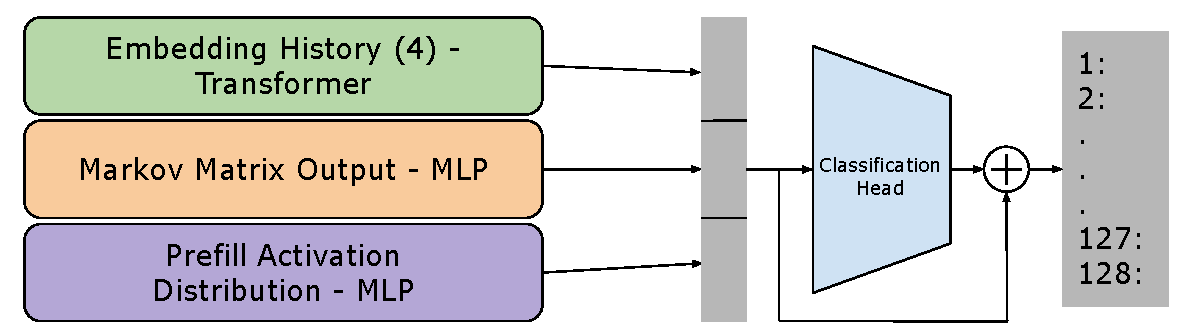
\includegraphics[width=\columnwidth]{figures/predictor_arch (1)_cropped.pdf}
    \vspace{-10pt}
    \caption{ExpertAhead Predictor Architecture}
    \label{fig:expertAhead_pred_arch}
    \vspace{-5pt}
\end{figure}

\subsubsection{Model Training Procedure}

Training data is collected by feeding chunks from the WikiText-103 training set \cite{merity2016pointersentinelmixturemodels} as prompts to Qwen3-30B-A3B-AWQ and recording the hidden-state embeddings and expert-activation traces during prefill and greedy decode. One predictor is trained independently per layer and per stride $S$.

\subsubsection{Runtime Integration}
\label{sec:prefetch_runtime}
Every $S$ decode steps, the predictor asynchronously ranks experts for the next $S$ tokens. Memory-resident experts among the top-$B$ predictions have their timestamps refreshed to prevent eviction. Non-resident experts are assigned victim slots via a least-frequently-recently-used (LFRU) policy and fetched via parallel, asynchronous SSD loads. Cache misses during actual routing trigger blocking loads, and any incomplete prefetch requests are discarded before the next predictor invocation to prevent stale workload backlog.

\subsection{Cache-Conditional Expert Selection}
To reduce the total number of SSD loads, \citet{skliar2025mixturecacheconditionalexpertsefficient} proposes an implementation of cache-conditional expert selection, evaluated on a mobile SoC. The modified router logits are defined as:

\begin{equation}
    \label{eq:top_j}
    z' = z + \lambda \cdot \Delta_{avg} \cdot \tilde{m}_t
\end{equation}


where $z$ are the original router logits, $\lambda$ is a tunable cache-bias strength parameter, and $\tilde{m}_t$ is a binary cache-residency mask indicating whether each expert is currently resident in system memory. The scaling factor $\Delta_{avg}$ normalizes the cache bias relative to the natural spread of the router logits, computed as an exponentially weighted moving average across forward passes.

In this work, we use $\lambda \in \{0,1\}$ and compare different values for top-J expert selection: the $J$ highest-scoring experts selected by the router are always activated, while the remaining $K-J$ expert slots become eligible for substitution with cache-resident experts to reduce SSD traffic. 


\subsection{Target Hardware}

We evaluate our methods on an AMD Ryzen AI 9 HX 370 (Strix Point) SoC. It includes a 12-core Zen 5 CPU and an AMD Radeon 890M integrated GPU sharing 28 GB of unified memory ($\sim$120 GB/s peak) and a peak achievable SSD bandwidth of $\sim$1.5 GB/s measured with an expert loading benchmark.
% \newpage
\section{Experiments}

\subsection{Predictor Input Feature Ablation Study} \label{sec:ablation_study}

This ablation study aims to identify an effective predictor architecture by exploring three primary dimensions:
\begin{enumerate}
    \item \textbf{Input Features}: We consider prior expert usage traces (Markov transition matrix), current/previous token embeddings, and prefill expert activation distributions.
    \item \textbf{Embedding Processor Architecture}:  A standard MLP versus a lightweight 2-layer, 4-head Transformer encoder.
    \item \textbf{Context History ($H$)}: Number of previous embeddings
\end{enumerate}

Performance is measured via Recall@B (fraction of activated experts within the next $S$ tokens captured in the top-$B$ predictions) and Precision@B (fraction of prefetched experts ultimately activated). Higher Recall@B reduces blocking SSD loads, while higher Precision@B minimizes wasted memory bandwidth.


Table~\ref{tab:arch_ablation_b16} shows that increasing the token embedding history and using a transformer instead of an equal-parameter-count MLP consistently increases performance. 


\begin{table}[h]
\centering
\caption{Recall and Precision (\%) at $B=16$. Embeddings only.}
\label{tab:arch_ablation_b16}
\begin{tabular}{l|cc|cc|cc}
\toprule
& \multicolumn{2}{c|}{\textbf{MLP Emb (H=1)}} & \multicolumn{2}{c|}{\textbf{MLP Emb (H=4)}} & \multicolumn{2}{c}{\textbf{Transformer (H=4)}} \\
\textbf{S} & \textbf{Recall} & \textbf{Prec} & \textbf{Recall} & \textbf{Prec} & \textbf{Recall} & \textbf{Prec} \\
\midrule
\textbf{1}  & 79.97 & 39.99 & 82.70 & 41.35 & 87.42 & 43.71 \\
\textbf{4}  & 49.84 & 71.76 & 51.49 & 74.27 & 54.75 & 79.06 \\
\textbf{8}  & 37.47 & 85.40 & 38.16 & 87.02 & 39.51 & 90.11 \\
\textbf{16} & 29.02 & 94.77 & 29.21 & 95.31 & 29.49 & 96.21 \\
\bottomrule
\end{tabular}
\end{table}

\begin{table}[h]
\centering
\caption{Transformer($H=4$) input feature ablation performance at budget $B=16$. Recall and Precision (\%)}
\label{tab:transformer_h4_ablation_b16}
\begin{tabular}{c|cc|cc|cc}
\toprule
\multirow{2}{*}{$S$} & \multicolumn{2}{c|}{\textbf{Base}} & \multicolumn{2}{c|}{\textbf{+Markov}} & \multicolumn{2}{c}{\textbf{+Markov \& Prefill}} \\
& Recall & Prec & Recall & Prec & Recall & Prec \\
\midrule
1 & 87.42 & 43.71 & 87.63 & 43.81 & 87.76 & 43.88 \\
4 & 54.75 & 79.06 & 54.88 & 79.26 & 55.02 & 79.45 \\
\bottomrule
\end{tabular}

\end{table}

Since larger strides involve more unique expert activations, the achievable Recall@B is constrained by the prefetch budget. For example, at a stride of 16 tokens, the median number of unique experts used by each layer is 38.
A budget of B=16 therefore has a theoretical maximum recall of 16/38 $\approx$ 42\%, although it may achieve a precision of up to 100\%.

Across all tested strides and budgets, the transformer-based architecture with $H=4$ outperforms the MLP-based architecture with $H=1$ by up to 7 \% in both recall and precision. Furthermore, incorporating the Markov prior and prefill distribution branches into either architecture provides small but consistent performance improvements. We show the effect of these branches on the Transformer ($H=4$) in Table~\ref{tab:transformer_h4_ablation_b16}. The marginal memory overhead of these feature branches is negligible, amounting to approximately 44~KB of trainable parameters per branch. Therefore, ExpertAhead uses a transformer with $H=4$ for the embedding branch, together with the Markov prior and prefill distribution features, as shown in Figure~\ref{fig:expertAhead_pred_arch}.

\subsection{Predictor Parameters} \label{sec:predictor_stride}
We define window recall as the percentage of experts out of the set that are used to generate the subsequent $S$ tokens (i.e. \{$t+1$, $t+S$\} where $t$ is the current token), that are predicted. Window precision is the percentage of predicted experts that are used over that window. For $C=48$, several combinations of strides and prefetch budgets are evaluated to find the resulting window precision $\pi$, window recall $\rho$, and throughput (TPS). An LFRU cache management policy is used. The baseline evicts a random inactive expert when we need to load an expert from SSD. We use 5 prompts based on the WikiText-103 test set and generate 80 tokens.



\begin{figure}[h]
    \centering
    \includegraphics[width=\columnwidth]{figures/tps_vs_recall_precision_C48.png}
    \vspace{-15pt}
    \caption{Recall-Precision vs Relative Throughput. $C=48$}
    \label{fig:expertAhead_c48}
    \vspace{-5pt}
\end{figure}

Figure~\ref{fig:expertAhead_c48} illustrates the tradeoffs between the independent variables $C$, $S$, $B$ and how they interact with dependent variables $\pi$, $\rho$, and the decode throughput (TPS).

Overall, throughput peaks at ($69\%$ recall, $63\%$ precision) for a stride of $S=5$ with budget $B=24$ ($1.39\times$ baseline). Interestingly, there is clear window recall-precision clustering across strides and budgets. This illustrates how $B$ and $C$, and the resulting $\pi$ and $\rho$ impact throughput with respect to the precision and recall constraints detailed in Section~\ref{list:constraints}.


\subsection{Perplexity Impact of Cache-Conditional Routing}
\label{sec:perplexity_degradation}
Cache-conditional routing improves throughput by substituting lower-priority SSD-resident experts with cache-resident experts, reducing total SSD loads, but modifies the router output and may therefore reduce model quality. We evaluate this tradeoff by varying the number of preserved top-$J$ experts and recording the change in perplexity score relative to using all router-selected experts.

\begin{table}[h]
    \centering
    \caption{Relative ($J=8$) Perplexity Change from changing $J$}
    \label{tab:perplexity_change}
    \begin{tabular}{lccccc}
    \toprule
    \textbf{Cache Size} & \textbf{$J=3$} & \textbf{$J=4$} & \textbf{$J=5$} & \textbf{$J=6$} & \textbf{$J=7$} \\
    \midrule
    $C = 16$ & +20.82\% & +8.46\% & +3.41\% & +1.36\% & -0.03\%  \\
    $C = 32$ & +13.00\% & +6.07\% & +2.26\% & +0.78\% & +0.03\%  \\
    $C = 48$ & +9.68\% & +4.07\% & +1.61\% & +0.50\% & +0.20\%  \\
    $C = 64$ & +6.51\% & +3.07\% & +1.18\% & +0.32\% & -0.04\%  \\
    \bottomrule
    \end{tabular}
\end{table}

As the cache size increases, there is a greater probability that an expert with a comparable router score is already in the cache, so the average increase in perplexity becomes smaller as the cache size increases for a given $J$.

\subsection{Cache Eviction Policy}
When managing the expert cache, an eviction policy must be chosen. \citet{skliar2025mixturecacheconditionalexpertsefficient} and \citet{eliseev2023fastinferencemixtureofexpertslanguage} both evict the least-recently used experts, while FlashMoE~\cite{kim2026flashmoereducingssdio} uses an ML-based policy. Although the eviction policy is reactive, it remains an important dimension of SSD-backed MoE inference. At $C$=64, decode throughput with an LFRU policy outperforms a policy evicting the most-recently-used expert by 1.75$\times$ and an LRU policy by 1.03$\times$. For our random eviction baseline, we use a policy where a random inactive expert is selected for eviction.


\subsection{End-to-End System Evaluation}

\begin{figure*}[t]
    \centering
    \includegraphics[width=2\columnwidth]{figures/expert_ahead_evaluation_random_cropped.png}
    \vspace{-10pt}
    \caption{End-to-End Comparison of Acceleration Techniques. Normalized to equal-memory cache with random eviction. ExpertAhead predictor outperforms Cross-Layer~\cite{eliseev2023fastinferencemixtureofexpertslanguage} at all measured cache sizes. ExpertAhead-CC adds prediction to Cache-Conditional~\cite{skliar2025mixturecacheconditionalexpertsefficient} which improves decode throughput with no additional perplexity change over \cite{skliar2025mixturecacheconditionalexpertsefficient} }
    \label{fig:expertAhead_results}
    \vspace{-5pt}
\end{figure*}

\begin{table*}[t]
\centering

\resizebox{\textwidth}{!}{%
\begin{tabular}{lcccccccccccccccc}
\toprule

&
\multicolumn{4}{c}{$\mathbf{C=16}$} &
\multicolumn{4}{c}{$\mathbf{C=32}$} &
\multicolumn{4}{c}{$\mathbf{C=48}$} &
\multicolumn{4}{c}{$\mathbf{C=64}$} \\

\cmidrule(lr){2-5}
\cmidrule(lr){6-9}
\cmidrule(lr){10-13}
\cmidrule(lr){14-17}

\textbf{Method}
&
\textbf{$S/B/J$} &
\textbf{TPS} &
\textbf{SSD} &
\textbf{Rand}
&
\textbf{$S/B/J$} &
\textbf{TPS} &
\textbf{SSD} &
\textbf{Rand}
&
\textbf{$S/B/J$} &
\textbf{TPS} &
\textbf{SSD} &
\textbf{Rand}
&
\textbf{$S/B/J$} &
\textbf{TPS} &
\textbf{SSD} &
\textbf{Rand}
\\

\midrule

SSD Streaming
&
-- & 1.30 & 1.00$\times$ & 0.53$\times$
&
-- & 1.30 & 1.00$\times$ & 0.38$\times$
&
-- & 1.30 & 1.00$\times$ & 0.29$\times$
&
-- & 1.30 & 1.00$\times$ & 0.23$\times$
\\

Random Eviction
&
--/--/-- & 2.44 & 1.88$\times$ & 1.00$\times$
&
--/--/-- & 3.44 & 2.65$\times$ & 1.00$\times$
&
--/--/-- & 4.49 & 3.45$\times$ & 1.00$\times$
&
--/--/-- & 5.69 & 4.38$\times$ & 1.00$\times$
\\

Oracle Predictor
&
2/--/-- & 4.36 & 3.36$\times$ & 1.79$\times$
&
1/--/-- & 7.91 & 6.09$\times$ & 2.30$\times$
&
1/--/-- & 14.21 & 10.93$\times$ & 3.17$\times$
&
1/--/-- & 17.69 & 13.61$\times$ & 3.11$\times$
\\

\midrule

Cross-Layer ~\cite{eliseev2023fastinferencemixtureofexpertslanguage}
&
--/8/-- & 2.24 & 1.72$\times$ & 0.92$\times$
&
--/6/-- & 3.47 & 2.67$\times$ & 1.01$\times$
&
--/2/-- & 5.18 & 3.99$\times$ & 1.16$\times$
&
--/2/-- & 7.35 & 5.66$\times$ & 1.29$\times$
\\

Cache-Conditional~\cite{skliar2025mixturecacheconditionalexpertsefficient}
&
--/--/5 & 3.47 & 2.67$\times$ & 1.42$\times$
&
--/--/5 & 5.44 & 4.18$\times$ & 1.58$\times$
&
--/--/5 & 8.17 & 6.29$\times$ & 1.82$\times$
&
--/--/5 & 10.97 & 8.44$\times$ & 1.93$\times$
\\

\midrule

\textbf{ExpertAhead}
&
2/4/-- & 2.62 & \textbf{2.02$\times$} & \textbf{1.08$\times$}
&
2/8/-- & 3.98 & \textbf{3.06$\times$} & \textbf{1.16$\times$}
&
5/24/-- & 6.19 & \textbf{4.77$\times$} & \textbf{1.38$\times$}
&
6/36/-- & 9.40 & \textbf{7.24$\times$} & \textbf{1.65$\times$}
\\

\textbf{ExpertAhead-CC}
&
1/4/5 & 3.52 & \textbf{2.71$\times$} & \textbf{1.45$\times$}
&
1/8/5 & 5.95 & \textbf{4.58$\times$} & \textbf{1.73$\times$}
&
4/20/5 & 8.60 & \textbf{6.62$\times$} & \textbf{1.92$\times$}
&
6/36/5 & 11.66 & \textbf{8.97$\times$} & \textbf{2.05$\times$}
\\

\bottomrule
\end{tabular}
}
\caption{End-to-end throughput across different expert cache sizes ($C$). Speedups are reported relative to both the SSD Streaming baseline and the Random Eviction baseline. Cross-Layer  reproduces~\cite{eliseev2023fastinferencemixtureofexpertslanguage} and Cache-Conditional  reproduces~\cite{skliar2025mixturecacheconditionalexpertsefficient}. Oracle Predictor represents the theoretical upper bound with best-case perfect prediction. "-" is N/A. (10 prompts, 150 generated tokens each)}
\label{tab:end_to_end_results}
\end{table*}

\subsubsection{Oracle Predictor}
We use precomputed expert usage traces to implement an oracle predictor which achieves 100\% recall and precision. Compared to an SSD streaming baseline, where all experts are loaded from SSD for computation and immediately discarded, the oracle achieves \textbf{13.61$\times$} decode speedup while only storing half of the model's total experts in memory ($C=64$). SSD streaming only requires enough memory to store the active experts for a single layer at a time, so this is not an equal-memory comparison. $C=64$ requires 384$\times$ as much memory as SSD streaming. Compared to an equal-memory baseline with the random eviction policy, the oracle predictor achieves up to \textbf{3.11$\times$} decode speedup. 


\subsubsection{ExpertAhead and ExpertAhead-CC}
We directly compare ExpertAhead and ExpertAhead-CC against  prior works: cross-layer predictive prefetching \cite{eliseev2023fastinferencemixtureofexpertslanguage} and pure cache-conditional routing \cite{skliar2025mixturecacheconditionalexpertsefficient} as well as an equal-memory random eviction baseline and SSD streaming in Table~\ref{tab:end_to_end_results}. \cite{eliseev2023fastinferencemixtureofexpertslanguage,skliar2025mixturecacheconditionalexpertsefficient} both use an LRU policy. For cache-conditional, we set $\lambda=1$ and $J=5$. We use the same settings for ExpertAhead-CC. We use 10 WikiText-103-based prompts and generate 150 tokens per prompt, reporting average normalized speedups over a random eviction policy. The results across four expert cache sizes are shown in Table~\ref{tab:end_to_end_results} and Figure~\ref{fig:expertAhead_results}. As cache size increases, raw TPS for all methods increases. Across all cache sizes ExpertAhead consistently outperforms cross-layer prediction \cite{eliseev2023fastinferencemixtureofexpertslanguage} and ExpertAhead-CC outperforms cache-conditional \cite{skliar2025mixturecacheconditionalexpertsefficient}. Compared to SSD streaming, ExpertAhead achieves up to a $7.24\times$ lossless speedup, while ExpertAhead-CC achieves $8.97\times$ speedup with a 1.2\% perplexity increase at $C=64$. At $C=64$ compared to the random eviction baseline, \textbf{ExpertAhead achieves up to a $1.65\times$ lossless speedup, while ExpertAhead-CC achieves $2.05\times$ speedup with a 1.2\% perplexity increase}.

 % For cross-layer prediction, $B$ refers to the optimal measured number of staging slots for the cache size $C$.

While recent reactive cache optimizations like FlashMoE \cite{kim2026flashmoereducingssdio} report a 7\% speedup over LRU for the base Qwen3-30B-A3B model for SSD-backed inference, our results for the quantized Qwen3-30B-A3B-AWQ yield significantly higher gains, validating our prediction-focused approach to SSD-backed decode acceleration. 

% This design point is also favorable relative to speculative decoding under an equal-memory comparison. Assume an expert cache of 8 experts per layer and additional memory which can be used introduce a draft model whose experts are one-quarter the size of the target model's experts (while sharing all other parameters \cite{wang2025moespeqspeculativequantizeddecoding}) or to expand the expert cache by 32 experts per layer, because 128 experts at $\frac{1}{4}$ the size is 32 at original size..
This design point is also favorable relative to speculative decoding under an equal-memory comparison. Assume an expert cache of 8 experts per layer and additional memory that can either be used to introduce a draft model whose experts are one-quarter the size of the target model's experts (while sharing all other parameters \cite{wang2025moespeqspeculativequantizeddecoding}) or to expand the expert cache by 32 experts per layer. The memory footprint of the draft model's experts is equivalent to 32 full-size experts per layer, since the target model contains 128 experts per layer. Even if the draft model achieves perfect prediction, the former reaches 2.6 TPS, expanding the cache from 8 to 40 experts per layer achieves 4.4 TPS, 69\% faster than the draft model-based solution.

% This design point is also favorable relative to speculative decoding under an equal-memory comparison. Assume an expert cache of 8 experts per layer and additional memory that can either be used to introduce a draft model whose experts are one-quarter the size of the target model's experts (while sharing all other parameters \cite{wang2025moespeqspeculativequantizeddecoding}) or to expand the expert cache by 32 experts per layer. The memory footprint of the draft model's experts is equivalent to 32 full-size experts per layer, since the target model contains 128 experts per layer. Even if the draft model achieves perfect prediction, allocating the additional memory to the draft model reaches only 2.6 TPS. In contrast, allocating the same memory to expand the expert cache from 8 to 40 experts per layer achieves 4.4 TPS, 69\% faster than the draft model-based solution.

% This design point is also favorable relative to speculative decoding under an equal-memory comparison. Introducing a draft model whose experts are one-quarter the size of the target model's experts (while sharing all other parameters \cite{wang2025moespeqspeculativequantizeddecoding}) consumes approximately the same memory as 32 experts per layer. Even if this draft model achieved perfect prediction, allocating that memory to the draft model yields only 2.6 TPS, whereas allocating the same memory to expand the expert cache from 8 to 40 experts per layer achieves 4.4 TPS or 69\% faster. 

% This underscores that ExpertAhead's small size is essential as memory can be better used to increase expert-cache capacity than to store a draft model.
% \newpage
\section{Conclusion}
 We presented ExpertAhead, a lightweight cross-token transformer-based predictor designed for SSD-backed MoE inference on memory-constrained UMA edge platforms, and ExpertAhead-CC, which combines this predictor with cache-conditional expert selection. Motivated by the observation that a cross-token oracle predictor can achieve up to a 3.11$\times$ decode speedup over an equal-memory expert cache baseline, we designed a predictor that uses token embeddings, previous expert usage, and prefill expert distribution to predict expert activations across several future decoding steps. This approach occupies a design space between existing short-horizon and long-horizon prediction methods and is optimized for SSD-backed inference.  Against the same baseline, ExpertAhead achieves a 1.65$\times$ lossless speedup, and ExpertAhead-CC achieves 2.05$\times$ speedup with only a small increase in perplexity. These results confirm that predictive prefetching and cache-conditional routing address distinct dimensions of the SSD bottleneck: blocking loads and traffic volume, respectively, and that combining them yields greater throughput than either alone.  Together, ExpertAhead and ExpertAhead-CC occupy a favorable design point for SSD-backed MoE deployment on memory-constrained UMA edge devices.

 % Existing cross-layer prediction methods provide limited overlap to hide SSD loads despite high accuracy, while speculative decoding-based approaches trade away cache capacity for a second in-memory model; ExpertAhead's small footprint avoids this tradeoff.
% \newpage

\section{AI Use Disclosure}
AI tools \cite{Cursor,Antigravity,ChatGPT} assisted with coding and paper editing. The conceptualization, design, and analysis of all MoE experiments are the contributions of the human authors.

%%%%%%% -- PAPER CONTENT ENDS -- %%%%%%%%

%%
%% The next two lines define the bibliography style to be used, and
%% the bibliography file.
\newpage
\bibliographystyle{ACM-Reference-Format}
\bibliography{papers}




\end{document}
\endinput
%%
%% End of file `sample-sigconf.tex'.
